\section{Injections and surjections}
\secbegin{secInjectionsSurjections}
\index{injection|(}
\index{surjection|(}
\index{bijection|(}

To motivate some of the definitions to come, look at the dots ($\bullet$) and stars ($\star$) below. Are there more dots or more stars?
\begin{center}
\fitwidth{\begin{tikzpicture}
\foreach \x in {1,2,3,4,5,6,7,8,9,10,11,12,13,14,15,16,17,18,19}
  \node at (0.75*\x, 0.75) {$\bullet$};

\foreach \x in {1,2,3,4,5,6,7,8,9,10,11,12,13,14,15}
  \node at (0.75*\x, 0) {$\star$};
\end{tikzpicture}}
\end{center}

Pause for a second and think about how you knew the answer to this question.

Indeed, there are more dots than stars. There are a couple of ways to arrive at this conclusion:
\begin{enumerate}[(i)] 
\item You could count the number of dots, count the number of stars, and then compare the two numbers; or
\item You could notice that the dots and the stars are evenly spaced, but that the line of dots is longer than the line of stars.
\end{enumerate}
It is likely that you chose method (ii). In fact, it is likely that you haven't even counted the number of dots or the number of stars yet---and you don't need to! We can conclude that there are more dots than stars by simply pairing up dots with stars---we eventually run out of stars, and there are still dots left over, so there must have been more dots than stars.

\subsection*{Injectivity}

One way of formalising this act of pairing up stars with dots mathematically is to define a function $f : S \to D$ from the set $S$ of stars to the set $D$ of dots, where the value of $f$ at each star is the dot that it is paired with. We of course must do this in such a way that each dot is paired with at most one star:

\begin{center}
\fitwidth{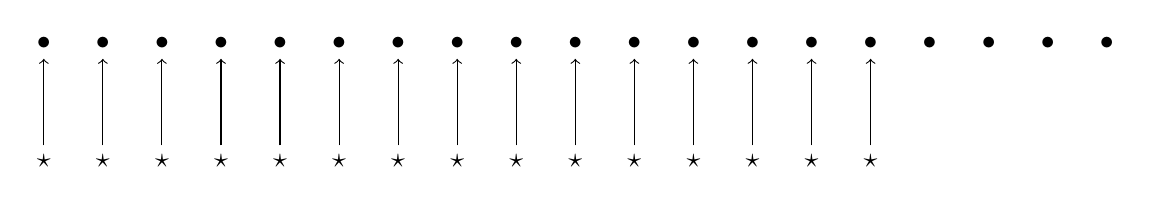
\begin{tikzpicture}
\foreach \x in {1,2,3,4,5,6,7,8,9,10,11,12,13,14,15,16,17,18,19}
  \node at (0.75*\x, 1.5) {$\bullet$};

\foreach \x in {1,2,3,4,5,6,7,8,9,10,11,12,13,14,15}
  \node at (0.75*\x, 0) {$\star$};

\foreach \x in {1,2,3,4,5,6,7,8,9,10,11,12,13,14,15}
  \draw [->] (0.75*\x, 0.2) -- (0.75*\x, 1.3);
\end{tikzpicture}}
\end{center}

It is a property of this function---called \textit{injectivity}---that allows us to deduce that there are more dots than stars.

Intuitively, a function $f : X \to Y$ is injective if it puts the elements of $X$ in one-to-one correspondence with the elements of a subset of $Y$---just like how the stars are in one-to-one correspondence with a subset of the dots in the example above.

\begin{definition}
\label{defInjective}\label{defInjection}
\index{function!injective (one-to-one)}
\index{injection}
A function $f : X \to Y$ is \textbf{injective} (or \textbf{one-to-one}) if
\[ \forall a,b \in X,\, f(a) = f(b) \Rightarrow a=b \]
An injective function is said to be an \textbf{injection}.
\end{definition}

\begin{strategy}[Proving a function is injective]
In order to prove that a function $f : X \to Y$ is injective, it suffices to fix $a,b \in X$, assume that $f(a)=f(b)$, and then derive $a=b$.
\end{strategy}

By contraposition, $f : X \to Y$ being injective is equivalent to saying, for all $a,b \in X$, if $a \ne b$, then $f(a) \ne f(b)$. This is usually less useful for \textit{proving} that a function is injective, but it does provide a good intuition---it says that $f$ sends distinct inputs to distinct outputs.

The following is a very simple example from elementary arithmetic:
\begin{example}
Define $f : \mathbb{Z} \to \mathbb{Z}$ by letting $f(x) = 2n+1$ for all $n \in \mathbb{Z}$. We'll prove that $f$ is injective. Fix $m, n \in \mathbb{Z}$, and assume that $f(m)=f(n)$. By definition of $f$, we have $2m+1=2n+1$. Subtracting $1$ yields $2m=2n$, and dividing by $2$ yields $m=n$. Hence $f$ is injective.
\end{example}

The following example is slightly more sophisticated.

\begin{proposition}
\label{propCompositeOfInjectionsIsInjection}
Let $f : X \to Y$ and $g : Y \to Z$ be functions. If $f$ and $g$ are injective, then $g \circ f$ is injective.
\end{proposition}
\begin{cproof}
Suppose that $f$ and $g$ are injective and let $a,b \in X$. We need to prove that
\[ (g \circ f)(a) = (g \circ f)(b) \quad \Rightarrow \quad a=b \]
So assume $(g \circ f)(a) = (g \circ f)(b)$. By definition of function composition, this implies that $g(f(a))=g(f(b))$. By injectivity of $g$, we have $f(a)=f(b)$; and by injectivity of $f$, we have $a=b$.
\end{cproof}

\begin{exercise}
Let $f : X \to Y$ and $g : Y \to Z$ be functions. Prove that if $g \circ f$ is injective, then $f$ is injective.
\end{exercise}

\begin{exercise}
Write out what it means to say a function $f : X \to Y$ is \textit{not} injective, and say how you would prove that a given function is not injective. Give an example of a function which is not injective, and use your proof technique to write a proof that it is not injective.
\end{exercise}

\begin{exercise}
For each of the following functions, determine whether it is injective or not injective.
\begin{itemize} 
\item $f : \mathbb{N} \to \mathbb{Z}$, defined by $f(n)=n^2$ for all $n \in \mathbb{N}$.
\item $g : \mathbb{Z} \to \mathbb{N}$, defined by $g(n)=n^2$ for all $n \in \mathbb{Z}$.
\item $h : \mathbb{N} \times \mathbb{N} \times \mathbb{N} \to \mathbb{N}$, defined by $h(x,y,z) = 2^x \cdot 3^y \cdot 5^z$ for all $x,y,z \in \mathbb{N}$.
\end{itemize}
\end{exercise}

\begin{exercise}
\label{exLinearPolynomialIsInjective}
Let $a,b \in \mathbb{R}$ with $b \ne 0$, and define $f : \mathbb{R} \to \mathbb{R}$ by $f(t) = a+bt$ for all $t \in \mathbb{R}$. Prove that $f$ is injective.
\end{exercise}

\subsection*{Surjectivity}

Let's revisit the rows of dots and stars that we saw earlier.  Beforehand, we made our idea that there are more dots than stars formal by proving the existence of an injection $f : S \to D$ from the set $S$ of stars to the set $D$ of dots.

However, we could have drawn the same conclusion instead from defining a function $D \to S$, which in some sense \textit{covers} the stars with dots---that is, every star is paired up with at least one dot.

\begin{center}
\fitwidth{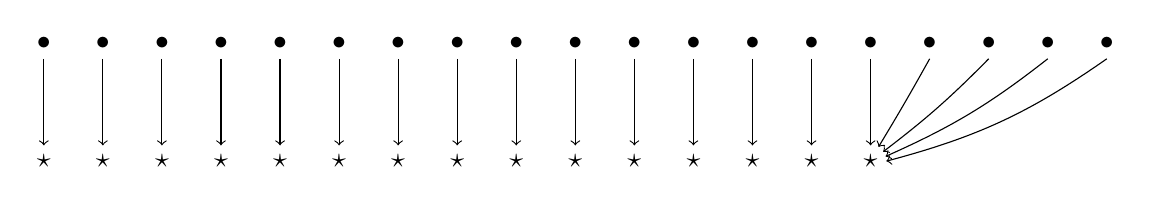
\begin{tikzpicture}
\foreach \x in {1,2,3,4,5,6,7,8,9,10,11,12,13,14,15,16,17,18,19}
  \node at (0.75*\x, 1.5) {$\bullet$};

\foreach \x in {1,2,3,4,5,6,7,8,9,10,11,12,13,14,15}
  \draw [->] (0.75*\x, 1.3) -- (0.75*\x, 0.2);

  \draw [->] (12, 1.3) to [bend left=1] (11.35, 0.18);
  \draw [->] (12.75, 1.3) to [bend left=4] (11.41, 0.12);
  \draw [->] (13.5, 1.3) to [bend left=7] (11.44, 0.06);
  \draw [->] (14.25, 1.3) to [bend left=10] (11.45, 0);

\foreach \x in {1,2,3,4,5,6,7,8,9,10,11,12,13,14,15}
  \node at (0.75*\x, 0) {$\star$};
\end{tikzpicture}}
\end{center}

This property is called \textit{surjectivity}---a function $f : X \to Y$ is surjective if every element of $Y$ is a value of $f$. This is made precise in \Cref{defSurjective}.

\begin{definition}
\label{defSurjective}\label{defSurjection}
A function $f : X \to Y$ is \textbf{surjective}\index{function!surjective}\index{surjection} (or \textbf{onto}) if
\[ \forall y \in Y,\ \exists x \in X,\ f(x) = y \]
A surjective function is said to be a \textbf{surjection}.
\end{definition}

\begin{strategy}
To prove that a function $f : X \to Y$ is surjective, it suffices to take an arbitrary element $y \in Y$ and, in terms of $y$, find an element $x \in X$ such that $f(x)=y$.

In order to find $x$, it is often useful to start from the equation $f(x)=y$ and derive some possible values of $x$. But be careful---in order to complete the proof, it is necessary to verify that the equation $f(x)=y$ is true for the chosen value of $x$.
\end{strategy}

\begin{example}
Fix $n \in \mathbb{N}$ with $n > 0$, and define a function $r : \mathbb{Z} \to \{ 0, 1, \dots, n-1 \}$ by letting $r(a)$ be the remainder of $a$ when divided by $n$ (see \Cref{thmDivisionPreliminary}). This function is surjective, since for each $k \in \{ 0, 1, \dots, n-1 \}$ we have $r(k)=k$.
\end{example}

\begin{exercise}
For each of the following pairs of sets $(X,Y)$, determine whether the function $f : X \to Y$ defined by $f(x)=2x+1$ is surjective.
\begin{enumerate}[(a)]
\item $X = \mathbb{Z}$ and $Y = \{ x \in \mathbb{Z} \mid x \text{ is odd} \}$;
\item $X = \mathbb{Z}$ and $Y = \mathbb{Z}$;
\item $X = \mathbb{Q}$ and $Y = \mathbb{Q}$;
\item $X = \mathbb{R}$ and $Y = \mathbb{R}$.
\end{enumerate}
\end{exercise}

\begin{exercise}
Let $f : X \to Y$ be a function. Find a subset $V \subseteq Y$ and a surjection $g : X \to V$ agreeing with $f$ (that is, such that $g(x)=f(x)$ for all $x \in X$).
\hintlabel{exSurjectiveCorestriction}{%
Recall \Cref{defImage}.
}
\end{exercise}

\begin{exercise}
Let $f : X \to Y$ be a function. Prove that $f$ is surjective if and only if $Y=f[X]$
\end{exercise}

\begin{exercise}
\label{exEpiMonoFactorisation}
Let $f : X \to Y$ be a function. Prove that there is a set $Z$ and functions
\[ p : X \to Z \quad \text{and} \quad i : Z \to Y \]
such that $p$ is surjective, $i$ is injective, and $f = i \circ p$.
\begin{backhint}
\hintref{exEpiMonoFactorisation}
If $Z$ were a subset of $Y$, then we could easily define an injection $i : Z \to Y$ by $i(z)=z$ for all $z \in Z$. Are there any subsets of $Y$ that are associated with a function whose codomain is $Y$?
\end{backhint}
\end{exercise}

\begin{exercise}
Let $f : X \to \mathcal{P}(X)$ be a function. By considering the set $B = \{ x \in X \mid x \not\in f(x) \}$, prove that $f$ is not surjective.
\hintlabel{exRussellSubset}{%
Note that $B \in \mathcal{P}(X)$. Prove that there does not exist $a \in X$ such that $B = f(a)$.
}
\end{exercise}

\subsection*{Bijectivity}

Bijective functions formalise the idea of putting sets into one-to-one correspondence---each element of one set is paired with exactly one element of another.

\begin{definition}
\label{defBijective}\label{defBijection}
A function $f : X \to Y$ is \textbf{bijective}\index{function!bijective} if it is injective and surjective. A bijective function is said to be a \textbf{bijection}\index{bijection}.
\end{definition}

\begin{prooftip}
To prove that a function $f$ is bijective, prove that it is injective and surjective.
\end{prooftip}

\begin{example}
\label{exDyadicRationalsBijection}
Let $D \subseteq \mathbb{Q}$ be the set of \textit{dyadic rational numbers}, that is
\[ D = \left\{ x \in \mathbb{Q} \ \bigg|\  x = \frac{a}{2^n} \text{ for some } a \in \mathbb{Z} \text{ and } n \in \mathbb{N} \right\} \]
Let $k \in \mathbb{N}$, and define $f : D \to D$ by $f(x)=\frac{x}{2^k}$. We will prove that $f$ is a bijection.
\begin{itemize}
\item (\textbf{Injectivity}) Fix $x,y \in D$ and suppose that $f(x)=f(y)$. Then $\frac{x}{2^k}=\frac{y}{2^k}$, so that $x=y$, as required.
\item (\textbf{Surjectivity}) Fix $y \in D$. We need to find $x \in D$ such that $f(x)=y$. Well certainly if $2^ky \in D$ then we have \[ f(2^ky)=\frac{2^ky}{2^k}=y \]
so it suffices to prove that $2^ky \in D$. Since $y \in D$, we must have $y=\frac{a}{2^n}$ for some $n \in \mathbb{N}$.
\begin{itemize}
\item If $k \le n$ then $n-k \in \mathbb{N}$ and so $2^ky=\frac{a}{2^{n-k}} \in D$.
\item If $k > n$ then $k-n>0$ and $2^ky = 2^{k-n}a \in \mathbb{Z}$; but $\mathbb{Z} \subseteq D$ since if $a \in \mathbb{Z}$ then $a=\frac{a}{2^0}$. So again we have $2^ky \in D$.
\end{itemize}
In any case we have $2^ky \in D$ and $f(2^ky)=y$, so that $f$ is surjective.
\end{itemize}
Since $f$ is both injective and surjective, it is bijective.
\end{example}

\begin{exercise}
\label{exIdentityBijection}
Let $X$ be a set. Prove that the identity function $\mathrm{id}_X : X \to X$ is a bijection.
\end{exercise}

\begin{exercise}
Let $n \in \mathbb{N}$ and let $\{ X_k \mid 1 \le k \le n \}$ be a family of sets. Prove by induction on $n$ that there is a bijection $\displaystyle \prod_{k=1}^{n+1} X_k \to \left( \prod_{k=1}^n X_k \right) \times X_n$.
\hintlabel{exProductOfSuccNSets}{%
To define the bijection, think about what the elements of the two sets look like: The elements of $\prod_{k=1}^{n+1} X_k$ look like $(a_1, a_2, \dots, a_n, a_{n+1})$, where $a_k \in X_k$ for each $1 \le k \le n+1$. On the other hand, the elements of $\left( \prod_{k=1}^n X_k \right) \times X_{n+1}$ look like $((a_1, a_2, \dots, a_n), a_{n+1})$.
}
\end{exercise}

\begin{exercise}
\label{exCompositeOfBijectionsIsBijection}
Let $f : X \to Y$ and $g : Y \to Z$ be bijections. Prove that $g \circ f$ is a bijection.
\end{exercise}

\subsection*{Inverses}

Our next goal is to characterise injections, surjections and bijections in terms of other functions, called \textit{inverses}.

Recall \Cref{defInjection}, which says that a function $f : X \to Y$ is injective if, for all $a,b \in X$, if $f(a)=f(b)$ then $a=b$.

\begin{exercise}
Let $f : X \to Y$ be a function. Prove that $f$ is injective if and only if
\[ \forall y \in f[X],\, \exists ! x \in X,\, y=f(x) \]
\end{exercise}

Thinking back to \Cref{secFunctions}, you might notice that this means that the logical formula `$y=f(x)$' defines a function $f[X] \to X$---specifically, if $f$ is injective then there is a function $g : f[X] \to X$ which is (well-)defined by specifying $x=g(f(x))$ for all $x \in X$. Thinking of $f$ as an \textit{encoding} function, we then have that $g$ is the corresponding \textit{decoding} function---decoding is possible by injectivity of $f$. (If $f$ were not injective then distinct elements of $X$ might have the same encoding, in which case we're stuck if we try to decode them!)

\begin{exercise}
\label{exEncodingPairs}
Define a function $e : \mathbb{N} \times \mathbb{N} \to \mathbb{N}$ by $e(m,n) = 2^m \cdot 3^n$. Prove that $e$ is injective. We can think of $e$ as encoding \textit{pairs} of natural numbers as single natural numbers---for example, the pair $(4,1)$ is encoded as $2^4 \cdot 3^1 = 48$. For each of the following natural numbers $k$, find the pairs of natural numbers encoded by $e$ as $k$:
\[ 1 \qquad 24 \qquad 7776 \qquad 59049 \qquad 396718580736 \]
\end{exercise}

In \Cref{exEncodingPairs}, we were able to decode any natural number of the form $2^m \cdot 3^n$ for $m,n \in \mathbb{N}$. This process of decoding yields a function
\[ d : \{ k \in \mathbb{N} \mid k=2^m \cdot 3^n \text{ for some } m,n \in \mathbb{N} \} \to \mathbb{N} \times \mathbb{N} \]
What would happen if we tried to decode a natural number not of the form $2^m \cdot 3^n$ for $m,n \in \mathbb{N}$, say $5$ or $100$? Well\dots{} it doesn't really matter! All we need to be true is that $d(e(m,n))=(m,n)$ for all $(m,n) \in \mathbb{N} \times \mathbb{N}$; the value of $d$ on other natural numbers is irrelevant.

\begin{definition}
\label{defLeftInverse}
\index{inverse!left inverse}
\index{left inverse}
Let $f : X \to Y$ be a function. A \textbf{left inverse} (or \textbf{post-inverse}) for $f$ is a function $g : Y \to X$ such that $g \circ f = \mathrm{id}_X$.
\end{definition}

\begin{example}
Let $e : \mathbb{N} \times \mathbb{N} \to \mathbb{N}$ be as in \Cref{exEncodingPairs}. Define a function $d : \mathbb{N} \to \mathbb{N} \times \mathbb{N}$ by
\[ d(k) = \begin{cases}
(m,n) & \text{if } k=2^m \cdot 3^n \text{ for some } m,n \in \mathbb{N} \\
(0,0) & \text{otherwise}
\end{cases} \]
Note that $d$ is well-defined by the fundamental theorem of arithmetic (\Cref{thmFTA}). Moreover, given $m,n \in \mathbb{N}$, we have
\[ d(e(m,n)) = d(2^m \cdot 3^n) = (m,n) \]
and so $d$ is a left inverse for $e$.
\end{example}

\begin{exercise}
\label{exIfHasLeftInverseThenInjective}
Let $f : X \to Y$ be a function. Prove that if $f$ has a left inverse, then $f$ is injective.
\end{exercise}

\Cref{exIfHasLeftInverseThenInjective} gives us a new strategy for proving that a function is injective.

\begin{strategy}[Proving a function is injective by finding a left inverse]
In order to prove that a function $f : X \to Y$ is injective, it suffices to find a function $g : Y \to X$ such that $g(f(x)) = x$ for all $x \in X$.
\end{strategy}

It would be convenient if the converse to \Cref{exIfHasLeftInverseThenInjective} were true---and it is, provided that we impose the condition that the domain of the function be inhabited.

\begin{proposition}
\label{propIfInjectiveThenHasLeftInverse}
Let $f : X \to Y$ be a function. If $f$ is injective and $X$ is inhabited, then $f$ has a left inverse.
\end{proposition}

\begin{cproof}
Suppose that $f$ is injective and $X$ is inhabited. Fix $x_0 \in X$---note that this element exists since $X$ is inhabited---and define $g : Y \to X$ as follows.
\[ g(y) = \begin{cases} x & \text{if } y=f(x) \text{ for some } x \in X \\ x_0 & \text{otherwise} \end{cases} \]
The only part of the specification of $g$ that might cause it to fail to be well-defined is the case when $y=f(x)$ for some $x \in X$. The reason why $g$ is well-defined is precisely injectivity of $f$: if $y=f(x)$ for some $x \in X$, then the value of $x \in X$ for which $y = f(x)$ is unique. (Indeed, if $a \in X$ satisfied $y=f(a)$, then we'd have $a=x$ by injectivity of $f$.)

So $g$ is indeed well-defined. To see that $g$ is a left inverse for $f$, let $x \in X$. Letting $y = f(x)$, we see that $y$ falls into the first case in the specification of $g$, so that $g(f(x)) = g(y) = a$ for the value of $a \in X$ for which $y = f(a)$---but as noted above, we have $a=x$ by injectivity of $f$.
\end{cproof}

\begin{exercise}
Let $f : X \to Y$ be a function with left inverse $g : Y \to X$. Prove that $g$ is a surjection.
\hintlabel{exLeftInversesAreSurjective}{%
This can be proved in a single sentence; if you find yourself writing a long proof, then there is an easier way.
}
\end{exercise}

We established a relationship between injections and left inverses in \Cref{exIfHasLeftInverseThenInjective,propIfInjectiveThenHasLeftInverse}, so it might come as no surprise that there is a relationship between surjections and \textit{right} inverses.

\begin{definition}
\label{defRightInverse}
\index{inverse!right inverse}
\index{right inverse}
Let $f : X \to Y$ be a function. A \textbf{right inverse} (or \textbf{pre-inverse}) for $f$ is a function $g : Y \to X$ such that $f \circ g = \mathrm{id}_Y$.
\end{definition}

\begin{example}
Define $f : \mathbb{R} \to \mathbb{R}^{\ge 0}$ by $f(x)=x^2$. Note that $f$ is surjective, since for each $y \in \mathbb{R}^{\ge 0}$ we have $\sqrt{y} \in \mathbb{R}$ and $f(\sqrt{y}) = y$. However $f$ is not injective; for instance
\[ f(-1) = 1 = f(1) \]
Here are three right inverses for $f$:
\begin{itemize}
\item The positive square root function $g : \mathbb{R}^{\ge 0} \to \mathbb{R}$ defined by $g(y)=\sqrt{y}$ for all $y \in \mathbb{R}^{\ge 0}$. Indeed, for each $y \in \mathbb{R}^{\ge 0}$ we have
\[ f(g(y)) = f(\sqrt{y}) = (\sqrt{y})^2 = y \]
\item The negative square root function $h : \mathbb{R}^{\ge 0} \to \mathbb{R}$ defined by $h(y)=-\sqrt{y}$ for all $y \in \mathbb{R}^{\ge 0}$. Indeed, for each $y \in \mathbb{R}^{\ge 0}$ we have
\[ f(h(y)) = f(-\sqrt{y}) = (-\sqrt{y})^2 = y \]
\item The function $k : \mathbb{R}^{\ge 0} \to \mathbb{R}$ defined by
\[ k(y) = \begin{cases}
\sqrt{y} & \text{if } 2n \le y < 2n+1 \text{ for some } n \in \mathbb{N} \\
-\sqrt{y} & \text{otherwise}
\end{cases} \]
Note that $k$ is well-defined, and again $f(k(y)) = y$ for all $y \in \mathbb{R}^{\ge 0}$ since no matter what value $k(y)$ takes, it is equal to either $\sqrt{y}$ or $-\sqrt{y}$.
\end{itemize}
There are many more right inverses for $f$---in fact, there are infinitely many more!
\end{example}

\begin{exercise}
Let $f : X \to Y$ be a function. Prove that if $f$ has a right inverse, then $f$ is surjective.
\hintlabel{exIfHasRightInverseThenSurjective}{%
The proof is almost identical to \Cref{exLeftInversesAreSurjective}.
}
\end{exercise}

\begin{strategy}[Proving a function is surjective by finding a right inverse]
In order to prove that a function $f : X \to Y$ is surjective, it suffices to find a function $g : Y \to X$ such that $f(g(y)) = y$ for all $y \in Y$.
\end{strategy}

\subsection*{Interlude: the axiom of choice}

It would be convenient if the converse to \Cref{exIfHasRightInverseThenSurjective} were true---that is, if $f : X \to Y$ is surjective, then it has a right inverse. Let's examine what a proof of this fact would entail. The fact that $f : X \to Y$ is surjective can be expressed as
\[ \forall y \in Y,\, \exists x \in X,\, f(x) = y \]
A right inverse would be a function $g : Y \to X$, so by \Cref{defFunction}, it must satisfy the following condition
\[ \forall y \in Y,\, \exists ! x \in X,\, g(y) = x \]

The temptation is therefore to construct $g : Y \to X$ as follows. Let $y \in Y$. By definition of surjectivity, there exists some $x \in X$ such that $f(x) = y$---define $g(y)$ to be such an element $x$. Then we have $f(g(y)) = f(x) = y$, as required.

There is an extremely subtle---but important---issue with this construction.

By choosing $g(y)$ to be a fixed element of $X$ such that $f(x) = y$, we are assuming ahead of time that there is a mechanism for choosing, for each $y \in Y$, a unique element of $f^{-1}[\{y\}]$ to be the value of $g(y)$. In other words we are assuming that some statement $R(x,y)$ satisfies the property
\[ \forall y \in Y,\, \exists ! x \in X,\, [x \in f^{-1}[\{y\}] \wedge R(x,y)] \]
But by \Cref{defFunction}, this assumption is saying exactly that there exists a function $Y \to X$ that associates to each $y \in Y$ an element $x \in X$ such that $f(x) = y$.

To state this in plainer terms: we tried to prove that there exists a right inverse for $f$ by assuming that there exists a right inverse for $f$. Evidently, this is not a valid proof strategy.

Surprisingly, it turns out that neither the assumption that every surjection has a right inverse, nor the assumption that there exists a surjection with no right inverse, leads to a contradiction. As such, the assertion that every surjection has a right inverse is \textit{provably unprovable}, although the proof that it is unprovable is far beyond the scope of this textbook.

Nonetheless, the construction of a right inverse that we gave above didn't \textit{feel} like we were abusing the fabric of mathematics and logic.

The essence of the proof is that if a statement of the form $\forall a \in A,\, \exists b \in B,\, p(a,b)$ is true, then we should be able to define a function $h : A \to B$ such that $p(a,h(a))$ is true for all $a \in A$: the function $h$ `chooses' for each $a \in A$ a particular element $b = h(a) \in B$ such that $p(a,b)$ is true.

What makes this possible is to \textit{axiom of choice}, stated precisely below.

\begin{axiom}[Axiom of choice]
\label{axChoice}
\index{axiom of choice}
Let $\{ X_i \mid i \in I \}$ be a family of inhabited sets. Then there is a function $h : I \to \bigcup\limits_{i \in I} X_i$ such that $h(i) \in X_i$ for each $i \in I$.
\end{axiom}

There are reasons to keep track of the axiom of choice:
\begin{itemize}
\item The axiom of choice is perhaps the \textit{strangest} assumption that we make---most of the other axioms that we have stated have been `evidently true', but this is not the case for the axiom of choice;
\item There are fields of mathematics which require the translation of results about sets into results about other kinds of objects---knowing whether the axiom of choice is necessary to prove a result tells us whether this is possible;
\item The axiom of choice is highly non-constructive: if a proof of a result that does not use the axiom of choice is available, it usually provides more information than a proof of the same result that does use the axiom of choice.
\end{itemize}

With this in mind, when we need to invoke the axiom of choice to prove a result, we will mark the result with the letters {\small \textbf{AC}}. This can be freely ignored on first reading, but readers may find it useful when using this book as a reference at a later date.

\begin{propositionac}
\label{propUsingAC}
Let $X$ and $Y$ be sets and let $p(x,y)$ be a logical formula with free variables $x \in X$ and $y \in Y$. If $\forall x \in X,\, \forall y \in Y,\, p(x,y)$ is true, then there exists a function $h : X \to Y$ such that $\forall x \in X,\, p(x,h(x))$ is true.
\end{propositionac}

\begin{cproof}
For each $a \in X$, define $Y_a = \{ b \in Y \mid p(a,b) \}$. Note that $Y_a$ is inhabited for each $a \in X$ by the assumption that $\forall x \in X,\, \exists y \in Y,\, p(x,y)$ is true. Since $Y_a \subseteq Y$ for each $a \in X$, by the axiom of choice there exists a function $h : X \to Y$ such that $h(a) \in Y_a$ for all $a \in X$. But then $p(a,h(a))$ is true for each $a \in X$ by definition of the sets $Y_a$.
\end{cproof}

In light of \Cref{propUsingAC}, the axiom of choice manifests itself in proofs as the following proof strategy.

\begin{strategyac}[Making choices]
\label{strUsingAC}
If an assumption in a proof has the form $\forall x \in X,\, \exists y \in Y,\, p(x,y)$, then we may make a choice, for each $a \in A$, of a particular element $b = b_a \in B$ for which $p(a,b)$ is true.
\end{strategyac}

\subsection*{Back to inverses}

We now return to the converse of \Cref{exIfHasRightInverseThenSurjective}.

\begin{propositionac}
Every surjection has a right inverse.
\end{propositionac}

\begin{cproof}
Let $f : X \to Y$ be a surjection, and define $g : Y \to X$ as follows. Given $y \in Y$, define $g(y)$ to be a particular choice of $x \in X$ such that $f(x) = y$---note that there exists such an element $x \in X$ since $f$ is surjective, so $g$ exists by \Cref{strUsingAC}. But then by definition of $g$ we have $f(g(y)) = y$ for all $y \in Y$, so that $g$ is a surjection.
\end{cproof}

It seems logical that we might be able to classify bijections as being those functions which have a left inverse and a right inverse. We can actually say something stronger---the left and right inverse can be taken to be the same function! (In fact, \Cref{propLeftAndRightInversesAreEqual} establishes that they are necessarily the same function.)

\begin{definition}
\label{defInverse}
\index{inverse!two-sided}
\index{two-sided inverse}
Let $f : X \to Y$ be a function. A (\textbf{two-sided}) \textbf{inverse} for $f$ is a function $g : Y \to X$ which is both a left inverse and a right inverse for $f$.
\end{definition}

It is customary to simply say `inverse' rather than `two-sided inverse'.

\begin{example}
Let $D$ be the set of dyadic rational numbers, as defined in \Cref{exDyadicRationalsBijection}. There, we defined a function $f : D \to D$ defined by $f(x)=\frac{x}{2^k}$ for all $x \in D$, where $k$ is some fixed natural number. We find an inverse for $f$.

Define $g : D \to D$ by $g(x) = 2^kx$. Then
\begin{itemize}
\item $g$ is a left inverse for $f$. To see this, note that for all $x \in D$ we have
\[ g(f(x)) = g(\frac{x}{2^k}) = 2^k \cdot \frac{x}{2^k} = x \]
\item $g$ is a right inverse for $f$. To see this, note that for all $y \in D$ we have
\[ f(g(y)) = f(2^ky) = \frac{2^ky}{2^k} = y \]
\end{itemize}
Since $g$ is a left inverse for $f$ and a right inverse for $f$, it is a two-sided inverse for $f$.
\end{example}

\begin{exercise}
\label{exFindTwoSidedInverses}
The following functions have two-sided inverses. For each, find its inverse and prove that it is indeed an inverse.
\begin{enumerate}[(a)]
\item $f : \mathbb{R} \to \mathbb{R}$ defined by $f(x)=\frac{2x+1}{3}$.
\item $g : \mathcal{P}(\mathbb{N}) \to \mathcal{P}(\mathbb{N})$ defined by $g(X) = \mathbb{N} \setminus X$.
\item $h : \mathbb{N} \times \mathbb{N} \to \mathbb{N}$ defined by $h(m,n) = 2^m(2n+1)-1$ for all $m,n \in \mathbb{N}$.
\end{enumerate}
\begin{backhint}
\hintref{exFindTwoSidedInverses}
For part (c), don't try to write a formula for the inverse of $h$; instead, use the fundamental theorem of arithmetic.
\end{backhint}
\end{exercise}

In light of the correspondences between injections and left inverses, and surjections and right inverses, it may be unsurprising that there is a correspondence between \textit{bijections} and \textit{two-sided inverses}.

\begin{exercise}
\label{exBijectiveIffHasInverse}
Let $f : X \to Y$ be a function. Then $f$ is bijective if and only if $f$ has an inverse.
\end{exercise}

\begin{strategy}[Proving a function is bijective by finding an inverse]
In order to prove that a function $f : X \to Y$ is bijective, it suffices to find a function $g : Y \to X$ such that $g(f(x)) = x$ for all $x \in X$ and $f(g(y)) = y$ for all $y \in Y$.
\end{strategy}

When proving a function $f : X \to Y$ is bijective by finding an inverse $g : Y \to X$, it is important to check that $g$ is \textit{both} a left inverse \textit{and} a right inverse for $f$. If you only prove that $g$ is a left inverse for $f$, for example, then you have only proved that $f$ is injective!

It turns out that if a function has both a left and a right inverse, then they must be equal. This is the content of the following proposition.

\begin{proposition}
\label{propLeftAndRightInversesAreEqual}
Let $f : X \to Y$ be a function and suppose $\ell : Y \to X$ is a left inverse for $f$ and $r : Y \to X$ is a right inverse for $f$. Then $\ell=r$.
\end{proposition}
\begin{cproof}
The proof is deceptively simple:
\begin{align*}
\ell &= \ell \circ \mathrm{id}_Y && \text{by definition of identity functions} \\
&= \ell \circ (f \circ r) && \text{since $r$ is a right inverse for $f$} \\
&= (\ell \circ f) \circ r && \text{by \Cref{exCompositionIsAssociative}} \\
&= \mathrm{id}_X \circ r && \text{since $\ell$ is a left inverse for $f$} \\
&= r && \text{by definition of identity functions}
\end{align*}
\end{cproof}

There is some intuition behind why the left and right inverses of a function $f : X \to Y$ should be equal if they both exist.
\begin{itemize}
\item A left inverse $\ell : Y \to X$ exists only if $f$ is injective. It looks at each element $y \in Y$ and, if it is in the image of $f$, returns the (unique) value $x \in X$ for which $f(x)=y$.
\item A right inverse $r : Y \to X$ exists only if $f$ is surjective. It looks at each element $y \in Y$ and picks out one of the (possibly many) values $x \in X$ for which $f(x)=y$.
\end{itemize}
When $f$ is a bijection, every element of $Y$ is in the image of $f$ (by surjectivity), and is a value of $f$ at a unique element of $X$ (by injectivity), and so the left and right inverses are forced to return the same value on each input---hence they are equal.

It follows from \Cref{propLeftAndRightInversesAreEqual} that, for any function $f : X \to Y$, any two inverses for $f$ are equal---that is, every bijective function has a \textit{unique} inverse!

\begin{notation}
Let $f : X \to Y$ be a function. Write $f^{-1} : Y \to X$\nindex{functionInverse}{$f^{-1}$}{inverse function} to denote the (unique) inverse for $f$, if it exists.
\end{notation}

\begin{proposition}
Let $f : X \to Y$ be a bijection. A function $g : Y \to X$ is a left inverse for $f$ if and only if it is a right inverse for $f$.
\end{proposition}

\begin{cproof}
We will prove the two directions separately.
\begin{itemize}
\item ($\Rightarrow$) Suppose $g : Y \to X$ is a left inverse for $f$---that is, $g(f(x))=x$ for all $x \in X$. We prove that $f(g(y))=y$ for all $y \in Y$, thus establishing that $g$ is a right inverse for $f$. So let $y \in Y$. Since $f$ is a bijection, it is in particular a surjection, so there exists $x \in X$ such that $y=f(x)$. But then
\begin{align*}
f(g(y)) &= f(g(f(x))) && \text{since $y=f(x)$} \\
&= f(x) && \text{since $g(f(x))=x$} \\
&= y && \text{since $y=f(x)$}
\end{align*}
So indeed $g$ is a right inverse for $f$.
\item ($\Leftarrow$) Suppose $g : Y \to X$ is a right inverse for $f$---that is, $f(g(y))=y$ for all $y \in Y$. We prove that $g(f(x))=x$ for all $x \in X$, thus establishing that $g$ is a left inverse for $f$. So let $x \in X$. Letting $y = f(x)$, we have $f(g(y)) = y$ since $g$ is a right inverse for $f$. This says precisely that $f(g(f(x)) = f(x)$, since $y=f(x)$. By injectivity of $f$, we have $g(f(x))=x$, as required.
\end{itemize}
\end{cproof}

\begin{exercise}
\label{exInverseBijection}
Let $f : X \to Y$ be a bijection. Prove that $f^{-1} : Y \to X$ is a bijection.
\begin{backhint}
\hintref{exInverseBijection}
Use \Cref{exBijectiveIffHasInverse}.
\end{backhint}
\end{exercise}

\begin{exercise}
\label{exCompositeBijection}
Let $f : X \to Y$ and $g : Y \to Z$ be bijections. Prove that $g \circ f : X \to Z$ is a bijection, and write an expression for its inverse in terms of $f^{-1}$ and $g^{-1}$.
\end{exercise}

\begin{exercise}
Let $f : X \to A$ and $g : Y \to B$ be bijections. Prove that there is a bijection $X \times Y \to A \times B$, and describe its inverse.
\hintlabel{exCartesianProductOfBijections}{%
Define $h : X \times Y \to A \times B$ by $h(x,y) = (f(x), g(y))$ for all $x \in X$ and all $y \in Y$; find an inverse for $h$ in terms of the inverses of $f$ and $g$.
}
\end{exercise}

At the beginning of this section we motivated the definitions of injections, surjections and bijections by using them to compare two quantities (of dots and stars)---however, as you might have noticed, we have not yet actually proved that thais intuition aligns with reality. For example, how do we know that if there is an injection $f : X \to Y$ then $Y$ has at least as many elements as $X$?

Answering this seemingly simple question is surprisingly difficult and has different answers depending on whether the sets involved are finite or infinite. In fact, the words `finite', `infinite' and `size' are themselves defined in terms of injections, surjections and bijections! We therefore leave this task to future sections.

In \Cref{secFiniteSets}, we define what it means for a set to be finite and what the size of a finite set is (\Cref{defFiniteSet}), and then prove that the sizes of finite sets can be compared by finding an injection, surjection or bijection between them \Cref{thmJectionsAndSizeOfNaturalNumbers}.

Comparing the sizes of infinite sets, and even defining what `size' means for infinite sets, is another can of worms entirely and leads to some fascinating mathematics. For example, we can prove some counterintuitive results, such as the set $\mathbb{N}$ of natural numbers and the set $\mathbb{Q}$ of rational numbers have the same size. The journey down this rabbit hole begins in \Cref{chInfinity}.


\index{injection|)}
\index{surjection|)}
\index{bijection|)}